\documentclass{beamer}
\usetheme{Singapore}
\usepackage[utf8]{inputenc}
\usecolortheme{crane}
\usepackage{graphicx}
\usepackage{iwona}
\usepackage{hyperref}
\usepackage[ruled]{algorithm2e}
\usepackage{listings}

\lstset{language=Python,
basicstyle=\ttfamily\bfseries,
commentstyle=\color{red}\itshape,
stringstyle=\color{darkgreen},
showstringspaces=false,
keywordstyle=\color{blue}\bfseries}

\beamertemplatenavigationsymbolsempty

% defining styles for tikz
\usepackage{tikz}
\usetikzlibrary{shapes.geometric, arrows}
\tikzstyle{process} = [rectangle, minimum width=2cm, minimum height=1.5cm, text centered, text width=2.2cm, draw=black, fill=orange!80]
\tikzstyle{decision} = [diamond, minimum width=2cm, minimum height=1.5cm, text centered, text width=2.2cm, draw=black, fill=green!80]
\tikzstyle{arrow} = [thick,->,>=stealth]
\tikzstyle{boardclass} = [rectangle, minimum width=3.6cm, text width=3.6cm,minimum height=3.5cm, draw=black, fill=cyan!50]
\tikzstyle{squareclass} = [rectangle, minimum width=3.6cm, text width=3.6cm, minimum height=2cm, draw=black, fill=orange!50]
\tikzstyle{robotclass} = [rectangle, minimum width=3.6cm, minimum height=7.1cm, text width=3.6cm, draw=black, fill=green!50]
\tikzstyle{codebox} = [rectangle, minimum width = 2cm, draw=none, fill=none]
\tikzstyle{chooseaction} = [rectangle, minimum width=10cm, minimum height=1.2cm, draw=red, ultra thick, fill=none]
\tikzstyle{learning} = [rectangle, minimum width=10.5cm, minimum height=1cm, draw=red, ultra thick, fill=none]
\tikzstyle{movement} = [rectangle, minimum width=6cm, minimum height=0.4cm, draw=red, ultra thick, fill=none]
\tikzstyle{reset} = [rectangle, minimum width=10cm, minimum height=1.4cm, draw=red, ultra thick, fill=none]
\tikzstyle{stt} = [rectangle, draw=none, fill=none]





\setbeamerfont{caption}{size=\tiny}


\title
{Playing with Reinforcement Learning in Python}
\subtitle
{The Q-Learning Algorithm}
\author{Geraint Palmer}
\date{Python Namibia, 2015 \newline \href{http://python-namibia.org}{\tiny{http://python-namibia.org}}}



\begin{document}
\frame{\titlepage}

  % 1st slide, Auraya
  \begin{frame}
  	\frametitle{Auraya}
	\begin{figure}
		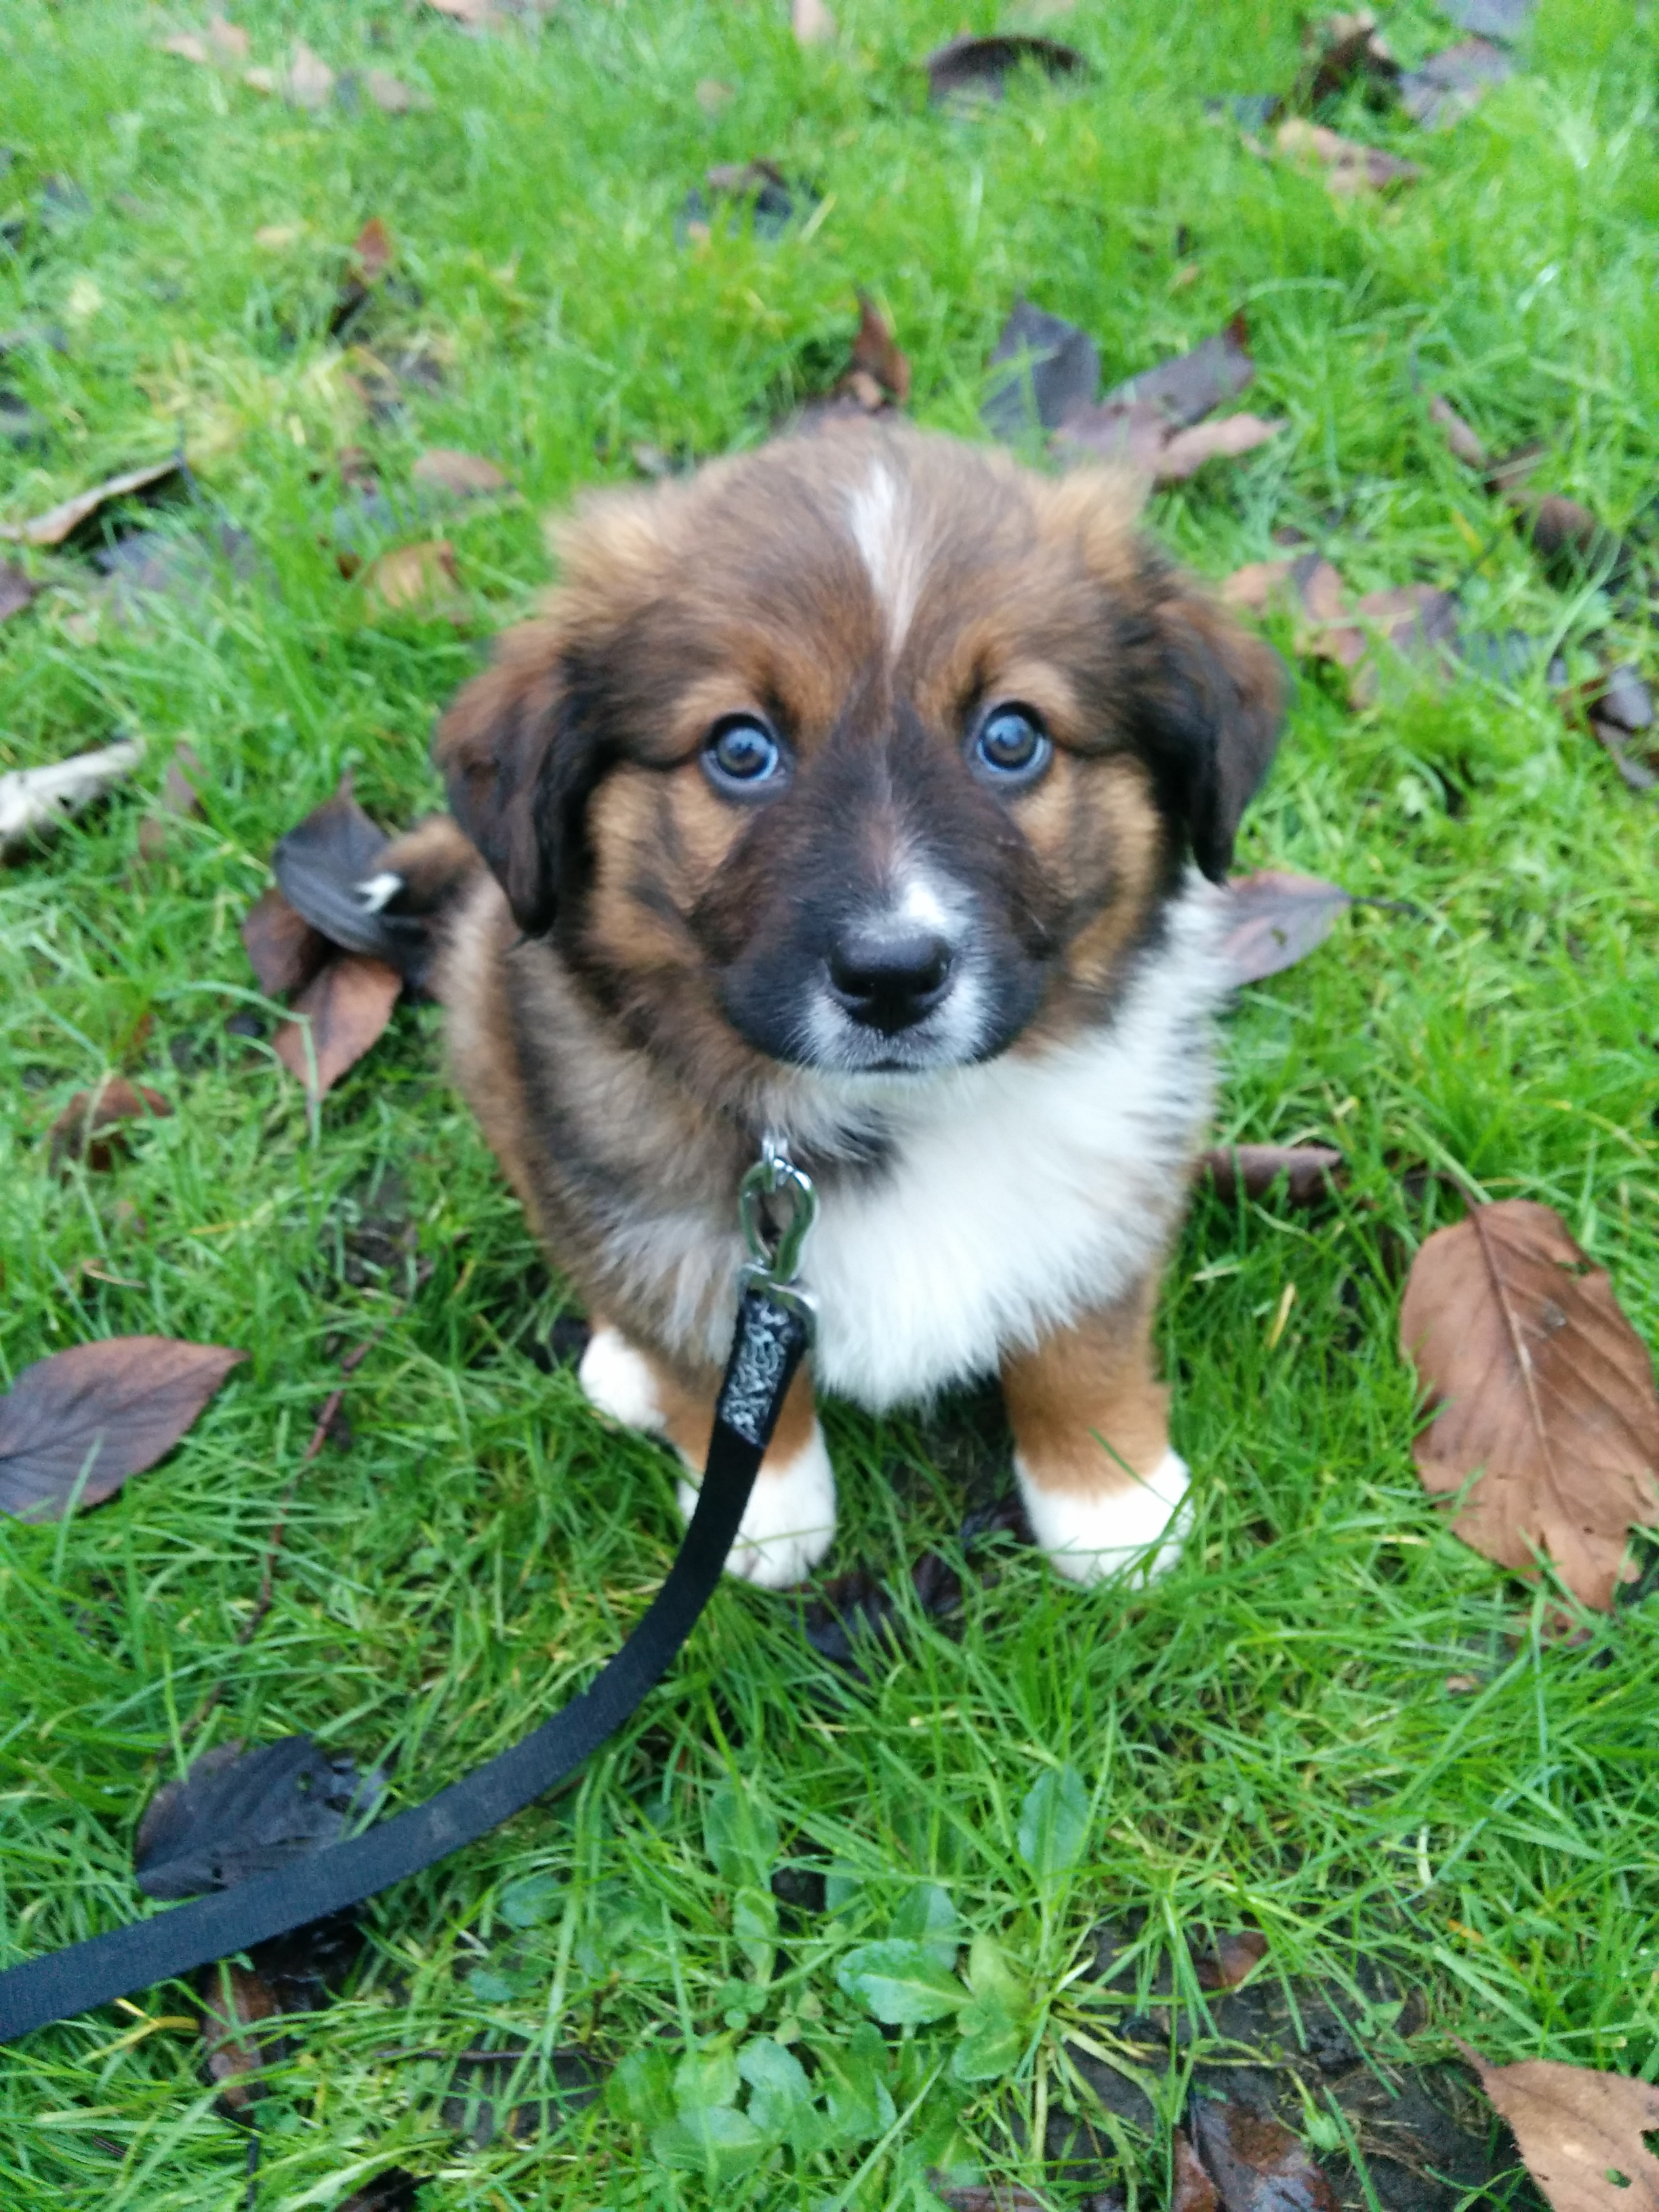
\includegraphics[width=5cm]{auraya}
	\end{figure}
  \end{frame}
  
  % 2nd slide, diagram of learning cycle, how to train a dog
  \begin{frame}
    \frametitle{How to train a dog?}
    \begin{center}
    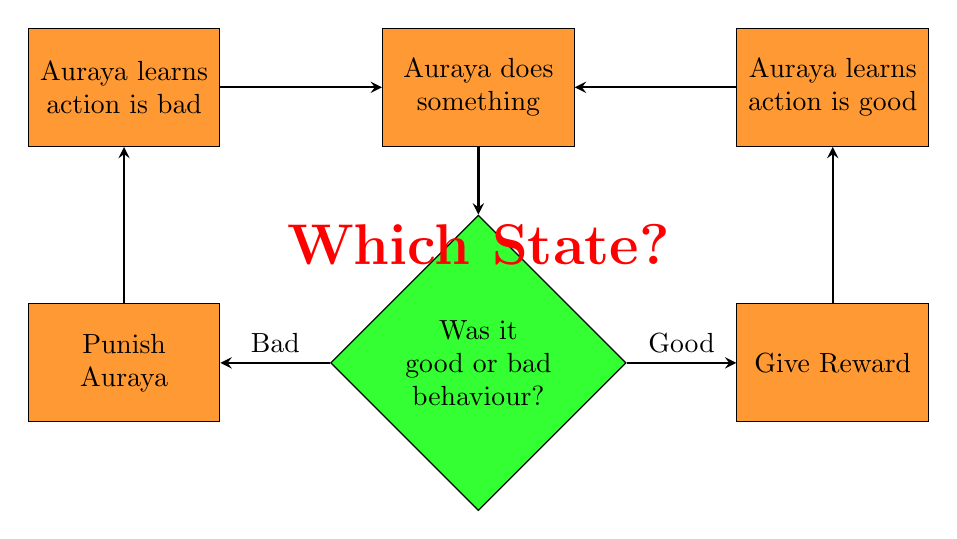
\begin{tikzpicture}[node distance=1.5cm]
		\node (dogact) [process] {Auraya does something};
		\node (learng) [process, right of=dogact, xshift=3cm] {Auraya learns action is good};
		\node (learnb) [process, left of=dogact, xshift=-3cm] {Auraya learns action is bad};
		\node (dec) [decision, below of=dogact, yshift=-2cm] {Was it good or bad behaviour?};
		\node (reward) [process, right of=dec, xshift=3cm] {Give Reward};
		\node (punish) [process, left of=dec, xshift=-3cm] {Punish Auraya};
		\draw [arrow] (dogact) -- (dec);
		\draw [arrow] (reward) -- (learng);
		\draw [arrow] (punish) -- (learnb);
		\draw [arrow] (learnb) -- (dogact);
		\draw [arrow] (learng) -- (dogact);
		\draw [arrow] (dec) -- node[anchor=south] {Good} (reward);
		\draw [arrow] (dec) -- node[anchor=south] {Bad} (punish);
		\pause
		\node (st) [stt, yshift=-2cm] {\huge{\textcolor{red}{\textbf{Which State?}}}};
    \end{tikzpicture}
    \end{center}
  \end{frame}
  
  % 3rd slide, the Q-learning algorithm
  \begin{frame}
  	\frametitle{The Q-learning Algorithm}
	\begin{center}
	\begin{algorithm}[H]
		\DontPrintSemicolon
		Set all $Q$ and $V$ values to 0\;
        \Repeat{convergence}{Observe the current state $s_t$\;
        Select and perform an action $a_t$\;
        Observe the reward $r(s_t, a_t)$\;
        Perform the following updates:\;
        \Indp $Q_{t+1} \leftarrow (1-\alpha)Q_t(s_t, a_t) + \alpha[r(s_t, a_t) + \gamma V_t(s_{t+1})]$\;
        $V_{t+1}(s) \leftarrow max_a Q_t(s, a)$\;
        }
    \end{algorithm}
    \end{center}
  \end{frame}
  
  
  % 4th slide, introduce the robot board game
  \begin{frame}
  	\frametitle{Rory The Robot}
	\begin{columns}[c]
	\column{0.7\textwidth}
		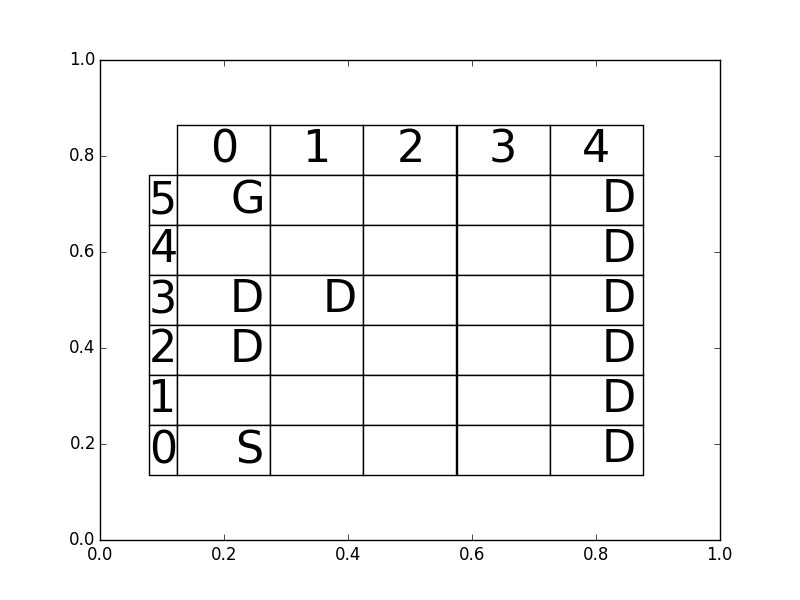
\includegraphics[width=8.5cm]{boardrory}
	\column{0.3\textwidth}
		\begin{center}
			
\includegraphics[width=2cm]{compass} \newline \newline \newline
			\pause
			\huge{\textbf{\textcolor{red}{only 85\% successful}}}
		\end{center}
	\end{columns}
  \end{frame}
  
  
  % 6th slide, classes
  \begin{frame}
  	\frametitle{Code Structure}
	\begin{center}
	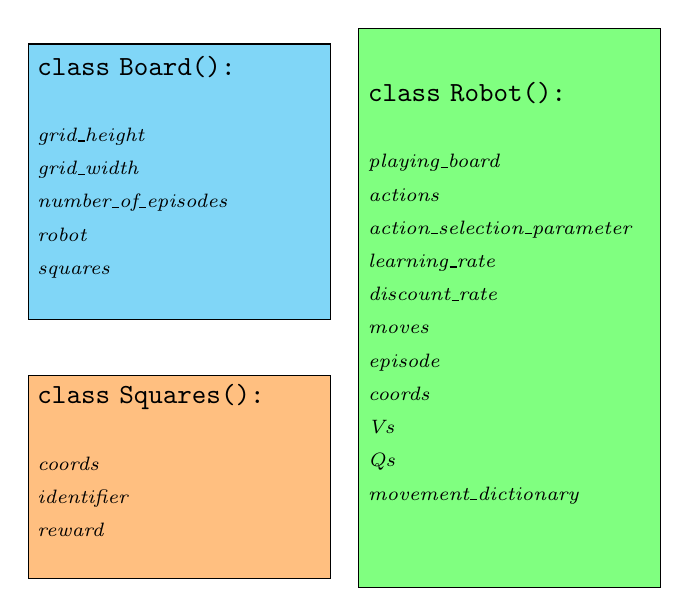
\begin{tikzpicture}
		\node (rcls) [robotclass] {\texttt{class Robot():} \newline
			\textit{\newline
			\scriptsize{playing\_board \newline
			actions \newline
			action\_selection\_parameter \newline
			learning\_rate \newline
			discount\_rate \newline
			moves \newline
			episode \newline
			coords \newline
			Vs \newline
			Qs \newline
			movement\_dictionary \newline}}};
		\node (bcls) [boardclass, left of=rcls, xshift=-3.2cm, yshift=1.6cm] {\texttt{class Board():} \newline
			\textit{\newline
			\scriptsize{grid\_height \newline
			grid\_width \newline
			number\_of\_episodes \newline
			robot \newline
			squares \newline
			}}};
		\node (scls) [squareclass, below of=bcls, yshift=-2.75cm] {\texttt{class Squares():} \newline
			\textit{\newline
			\scriptsize{coords \newline
			identifier \newline
			reward \newline
			}}};
	\end{tikzpicture}
	\end{center}
  \end{frame}
  
  % 6th slide, classes
  \begin{frame}
  	\frametitle{Code Structure}
	\begin{center}
	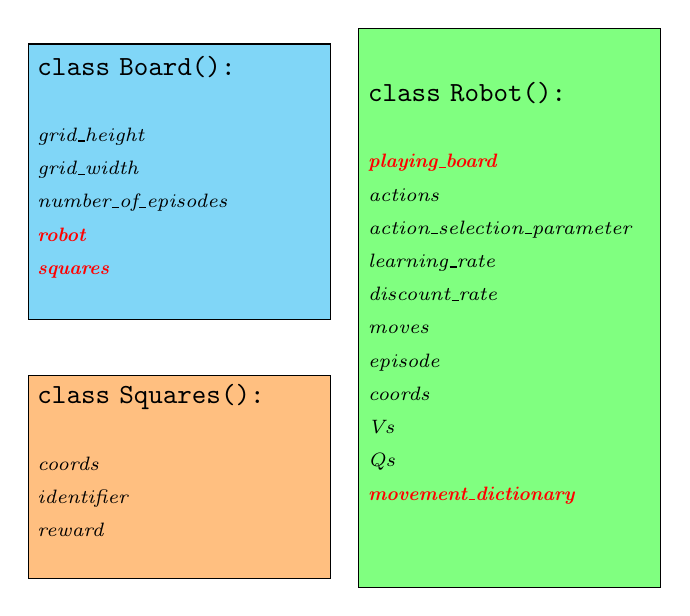
\begin{tikzpicture}
		\node (rcls) [robotclass] {\texttt{class Robot():} \newline
			\textit{\newline
			\scriptsize{\textcolor{red}{\textbf{playing\_board}} \newline
			actions \newline
			action\_selection\_parameter \newline
			learning\_rate \newline
			discount\_rate \newline
			moves \newline
			episode \newline
			coords \newline
			Vs \newline
			Qs \newline
			\textcolor{red}{\textbf{movement\_dictionary}} \newline}}};
		\node (bcls) [boardclass, left of=rcls, xshift=-3.2cm, yshift=1.6cm] {\texttt{class Board():} \newline
			\textit{\newline
			\scriptsize{grid\_height \newline
			grid\_width \newline
			number\_of\_episodes \newline
			\textcolor{red}{\textbf{robot \newline
			squares}} \newline
			}}};
		\node (scls) [squareclass, below of=bcls, yshift=-2.75cm] {\texttt{class Squares():} \newline
			\textit{\newline
			\scriptsize{coords \newline
			identifier \newline
			reward \newline
			}}};
	\end{tikzpicture}
	\end{center}
  \end{frame}

    % 7th slide, action selection
  \begin{frame}[fragile]
	\frametitle{Action Selection - Exploration vs Exploitation}
	\begin{center}
	$\epsilon$-Soft Policy
	\end{center}
	\lstset{language=Python,
				basicstyle=\tiny\ttfamily,
				commentstyle=\color{red},
				stringstyle=\color{orange},
				keywordstyle=\color{blue},
				frame=tb}

	\begin{lstlisting}
		def select_action(self, sqr):
		    """
		    Selects which action to take using the epsilon-soft action selection policy
		    """
		    rnd_num = random.random()
		    if rnd_num < 1 - self.action_selection_parameter:
		        return str(max(self.Qs[sqr], key=lambda x: self.Qs[sqr][x]))
		    return random.choice(self.actions)
	\end{lstlisting}
\end{frame}

    % 8th slide, Movement
  \begin{frame}[fragile]
	\frametitle{Movement}
	\lstset{language=Python,
				basicstyle=\tiny\ttfamily,
				commentstyle=\color{red},
				stringstyle=\color{orange},
				keywordstyle=\color{blue},
				frame=tb}

	\begin{lstlisting}
	def find_destination(self, sqr, action):
	   """
	   Chooses the new coordinates after taking an action, according to the faultiness
	   """
	   rnd_num = random.random()
	   sum_p, indx = 0, 0
	   while rnd_num > sum_p:
	      direction = self.actions[indx]
	      sum_p += self.transitions[action][indx]
	      indx += 1
	   return self.movement_dict[direction](sqr)
	\end{lstlisting}
\end{frame}
  

  
  % 9th slide, Learning
  \begin{frame}[fragile]
	\frametitle{Learning}
	\lstset{language=Python,
				basicstyle=\tiny\ttfamily,
				commentstyle=\color{red},
				stringstyle=\color{orange},
				keywordstyle=\color{blue},
				frame=tb}

	\begin{lstlisting}
		def Q_Learning(self, action, reward, sqr, new_sqr):
		    """
		    Updates Rory's Q and V values
		    """
		    self.Qs[sqr][action] = (
		        1-self.learning_rate)*self.Qs[sqr][action] + self.learning_rate*(
		        reward + self.discount_rate*self.Vs[new_sqr]
		        )
		    self.Vs[sqr] = max(self.Qs[sqr].values())
	\end{lstlisting}
\end{frame}
  
  
  
  
  
  
  
  % 10th slide, Simulation
  \begin{frame}[fragile]
	\frametitle{Simulation}
	\lstset{language=Python,
				basicstyle=\tiny\ttfamily,
				commentstyle=\color{red},
				stringstyle=\color{orange},
				keywordstyle=\color{blue},
				frame=tb}
	\begin{tikzpicture}
		\node (mycodebox) [codebox] {
	\begin{lstlisting}
		def simulate(self):
		    """
		    Simulates many episodes of the game while the robots learns the best policies
		    """
		    plt.ion()
		    self.show_board()
		    wait = raw_input('Press enter to continue.')
		    print 'Simulating .......'
		    while self.robot.episode < self.number_of_episodes:
			        action = self.robot.select_action(self.robot.coords)
			        new_coords = self.robot.find_destination(self.robot.coords, action)
			        self.robot.moves += 1

			        reward = self.squares[new_coords[1]][new_coords[0]].reward + (
				            self.squares[new_coords[1]][new_coords[0]].move_cost * self.robot.moves)
			        self.robot.Q_Learning(action, reward, self.robot.coords, new_coords)
			
			        self.robot.coords = new_coords

			        if (self.squares[new_coords[1]][new_coords[0]].identifier == 'Death' or 
				            self.squares[new_coords[1]][new_coords[0]].identifier == 'Goal'):
				            self.robot.moves = 0
				            self.robot.coords = tuple(self.starting_coords)
				            self.robot.episode += 1
		    self.update_results()
		    wait = raw_input('Simulated. Press enter to exit.')
	\end{lstlisting}
	};
	\only<2> \node (actionrectangle) [chooseaction, xshift=-0.4cm, yshift=0.8cm] {};
	\only<3> \node (learnrectangle) [learning, xshift=0.45cm, yshift = -0.3cm] {};
	\only<4> \node (moverectangle) [movement, xshift=-2.5cm, yshift=-1.05cm] {};
	\only<5> \node (resetrectangle) [reset, xshift=0.25cm, yshift=-2.12cm] {};
	\end{tikzpicture}
\end{frame}
  
  % 11th slide, demo
  \begin{frame}
  	\frametitle{Demo}
  \end{frame}
  
  % 12th slide, the learning rate alpha
  \begin{frame}
  	\frametitle{Learning Rate, $\alpha$}
	\center{Small $\alpha \implies$ historical rewards more important}
	\center{Large $\alpha \implies$ the latest reward more important}
	\begin{figure}
		\begin{minipage}{.32\textwidth}
			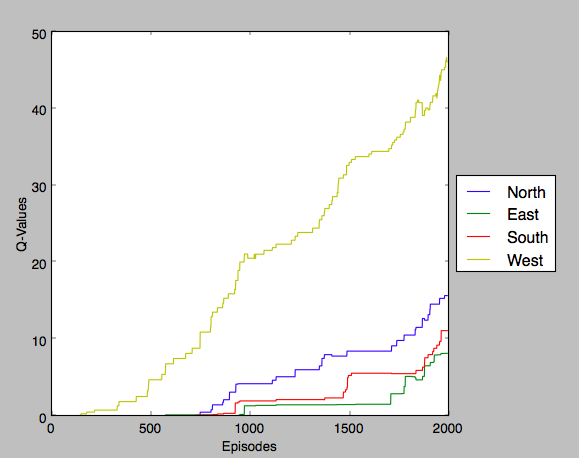
\includegraphics[width=3.4cm]{25a03g9}
				\caption{$\alpha = 0.03$}
		\end{minipage}
		\begin{minipage}{0.32\textwidth}
			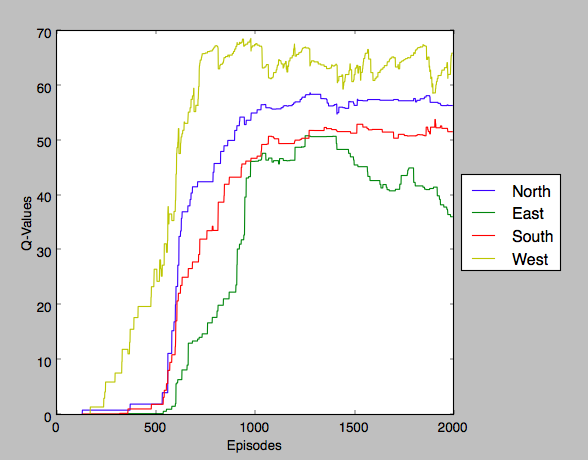
\includegraphics[width=3.4cm]{25a1g9}
				\caption{$\alpha = 0.1$}
		\end{minipage}
		\begin{minipage}{0.32\textwidth}
			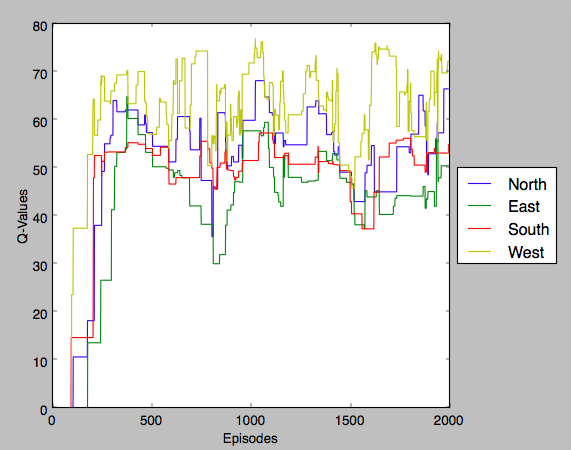
\includegraphics[width=3.4cm]{25a5g9}
				\caption{$\alpha = 0.5$}
		\end{minipage}
	\end{figure}
  \end{frame}
  
  % 13th slide, the discount rate beta
  \begin{frame}
  	\frametitle{Discount Rate, $\gamma$}
	\center{Small $\gamma \implies$ look for immediate rewards}
	\center{Large $\gamma \implies$ strive for long term rewards}
	\begin{figure}
		\begin{minipage}{.32\textwidth}
			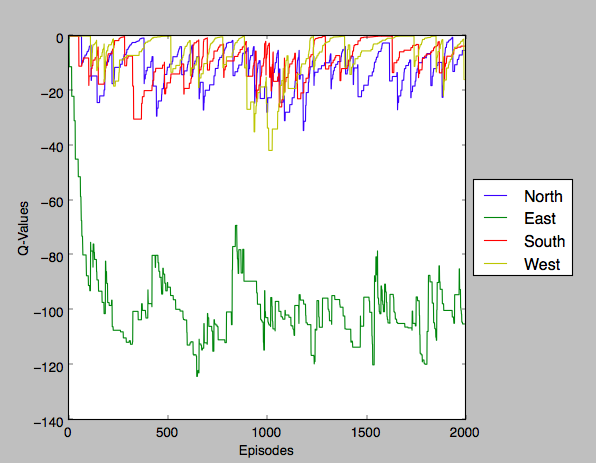
\includegraphics[width=3.4cm]{30a1g1}
				\caption{$\gamma = 0.1$}
		\end{minipage}
		\begin{minipage}{0.32\textwidth}
			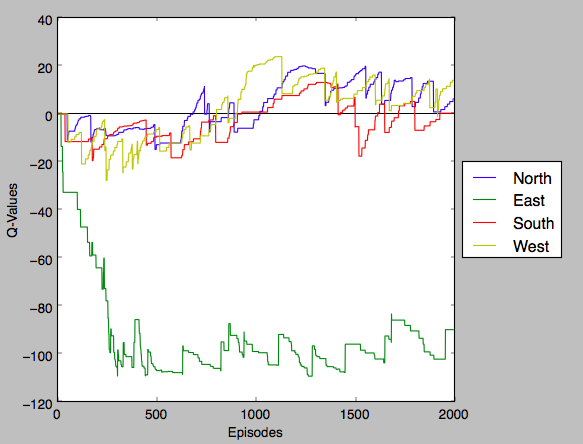
\includegraphics[width=3.4cm]{30a1g9}
				\caption{$\gamma = 0.9$}
		\end{minipage}
		\begin{minipage}{0.32\textwidth}
			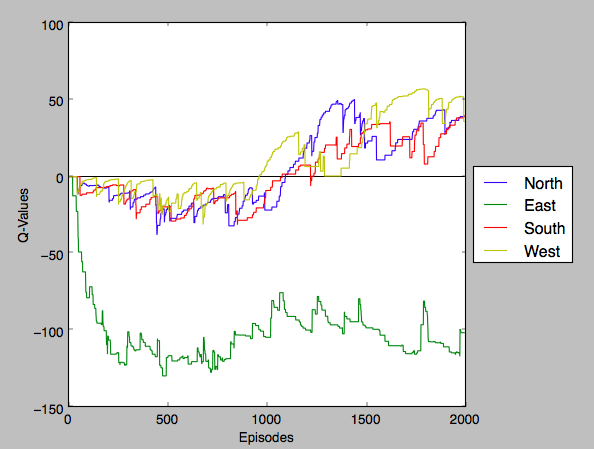
\includegraphics[width=3.4cm]{30a1g99}
				\caption{$\gamma = 0.99$}
		\end{minipage}
	\end{figure}
  \end{frame}
  
  % 14th slide, my phd
  \begin{frame}
  	\frametitle{Using RL in a Healthcare System}
	\begin{figure}
		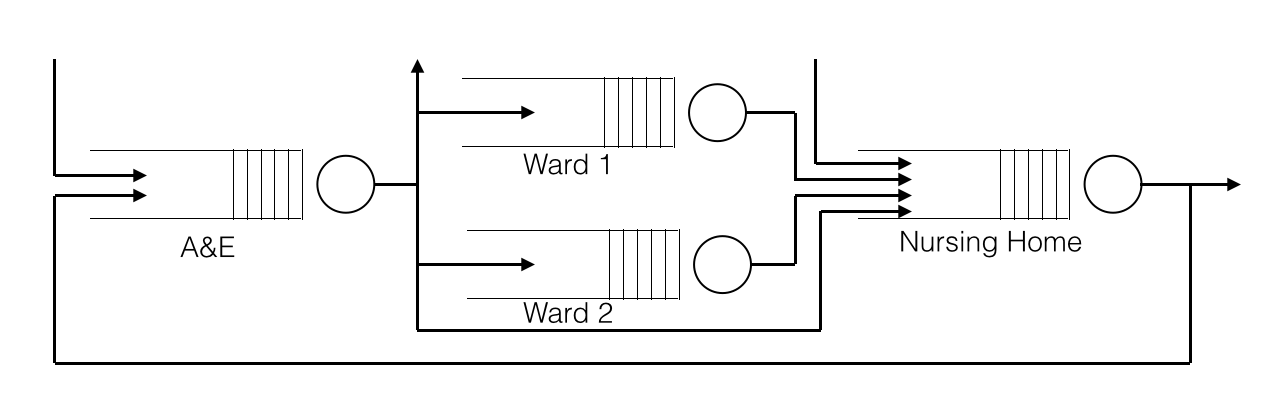
\includegraphics[width=11cm]{QueueingNetwork}
	\end{figure}
  \end{frame}
  
  % 15th slide, Links
  \begin{frame}
  	\frametitle{Links}
	\href{https://www.youtube.com/watch?v=CthhCy-1Jeg}{A robot learning to walk} \newline
	\href{https://www.youtube.com/watch?v=kM89G5dE-og}{A computer learning to play 'snake'} \newline
	\href{https://www.youtube.com/watch?v=zOgSC---rgM}{A virtual car learning not to crash} \newline
	\href{https://www.youtube.com/watch?v=X33xYf4UlVw}{An agent learning the shortest route through a maze} \newline
	\newline
	\href{https://github.com/geraintpalmer/Python_Namibia_2015}{https://github.com/geraintpalmer/Python\_Namibia\_2015}
	\end{frame}
  
\end{document}





